% Seminar 9: Prophet și TBATS
% Prezentare academică de calitate Harvard
% Program de licență, Academia de Studii Economice din București

\documentclass[9pt, aspectratio=169, t]{beamer}

% Standard 8mm margins for seminar slides
\setbeamersize{text margin left=8mm, text margin right=8mm}

%=============================================================================
% CONFIGURARE TEMĂ ȘI STIL
%=============================================================================
\usetheme{default}

% Color Palette (matching Redispatch PDF)
\definecolor{MainBlue}{RGB}{26, 58, 110}
\definecolor{AccentBlue}{RGB}{26, 58, 110}
\definecolor{IDAred}{RGB}{205, 0, 0}
\definecolor{DarkGray}{RGB}{51, 51, 51}
\definecolor{MediumGray}{RGB}{128, 128, 128}
\definecolor{LightGray}{RGB}{248, 248, 248}
\definecolor{VeryLightGray}{RGB}{235, 235, 235}
\definecolor{KeynoteGray}{RGB}{218, 218, 218}
\definecolor{SectionGray}{RGB}{120, 120, 120}
\definecolor{FooterGray}{RGB}{100, 100, 100}
\definecolor{Crimson}{RGB}{220, 53, 69}
\definecolor{Forest}{RGB}{46, 125, 50}
\definecolor{Amber}{RGB}{181, 133, 63}
\definecolor{Orange}{RGB}{230, 126, 34}
\definecolor{Purple}{RGB}{142, 68, 173}

% Gradient background (exact Keynote 315 gradient: white to RGB 218,218,218)
\setbeamertemplate{background}{%
    \begin{tikzpicture}[remember picture, overlay]
        \shade[shading=axis, shading angle=315,
        top color=white, bottom color=KeynoteGray]
        (current page.south west) rectangle (current page.north east);
    \end{tikzpicture}%
}
% Fallback solid color for compatibility
\setbeamercolor{background canvas}{bg=}

\setbeamercolor{palette primary}{bg=MainBlue, fg=white}
\setbeamercolor{palette secondary}{bg=MainBlue!85, fg=white}
\setbeamercolor{palette tertiary}{bg=MainBlue!70, fg=white}
\setbeamercolor{structure}{fg=MainBlue}
\setbeamercolor{title}{fg=IDAred}
\setbeamercolor{frametitle}{fg=IDAred, bg=}
\setbeamercolor{block title}{bg=MainBlue, fg=white}
\setbeamercolor{block body}{bg=VeryLightGray, fg=DarkGray}
\setbeamercolor{block title alerted}{bg=Crimson, fg=white}
\setbeamercolor{block body alerted}{bg=Crimson!8, fg=DarkGray}
\setbeamercolor{block title example}{bg=Forest, fg=white}
\setbeamercolor{block body example}{bg=Forest!8, fg=DarkGray}
\setbeamercolor{item}{fg=MainBlue}

% Footer colors (override Madrid theme blue)
\setbeamercolor{author in head/foot}{fg=FooterGray, bg=}
\setbeamercolor{title in head/foot}{fg=FooterGray, bg=}
\setbeamercolor{date in head/foot}{fg=FooterGray, bg=}
\setbeamercolor{section in head/foot}{fg=FooterGray, bg=}
\setbeamercolor{subsection in head/foot}{fg=FooterGray, bg=}

% Bullet styles (apply everywhere including blocks)
\setbeamertemplate{itemize item}{\color{MainBlue}$\boxdot$}
\setbeamertemplate{itemize subitem}{\color{MainBlue}$\blacktriangleright$}
\setbeamertemplate{itemize subsubitem}{\color{MainBlue}\tiny$\bullet$}
\setbeamertemplate{itemize/enumerate body begin}{\normalsize}
\setbeamertemplate{itemize/enumerate subbody begin}{\normalsize}

% Item spacing - compact style
\setlength{\leftmargini}{10pt}       % Level 1: minimal indent
\setlength{\leftmarginii}{10pt}      % Level 2: minimal additional indent
% Compact list spacing (zero extra space before/after lists in blocks)
\makeatletter
\def\@listi{\leftmargin\leftmargini \topsep 0pt \parsep 0pt \itemsep 0pt}
\def\@listii{\leftmargin\leftmarginii \topsep 0pt \parsep 0pt \itemsep 0pt}
\makeatother

\setbeamertemplate{navigation symbols}{}

%=============================================================================
% CUSTOM HEADLINE
%=============================================================================
\setbeamertemplate{headline}{%
    \vskip10pt%
    \hbox to \paperwidth{%
        \hskip0.5cm%
        {\small\color{FooterGray}\renewcommand{\hyperlink}[2]{##2}\insertsectionhead}%
        \hfill%
        \textcolor{FooterGray}{\small\insertframenumber}%
        \hskip0.5cm%
    }%
    \vskip4pt%
    {\color{FooterGray}\hrule height 0.4pt}%
}

%=============================================================================
% CUSTOM FOOTER
%=============================================================================
\usepackage{fontawesome5}

\setbeamertemplate{footline}{%
    {\color{FooterGray}\hrule height 0.4pt}%
    \vskip4pt%
    \hbox to \paperwidth{%
        \hskip0.5cm%
        \textcolor{FooterGray}{\small Analiza și Prognoza seriilor de timp}%
        \hfill%
        \raisebox{-0.1em}{%
            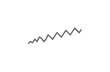
\begin{tikzpicture}[x=0.08em, y=0.08em, line width=0.4pt]
                \draw[FooterGray] (0,3) -- (1,4) -- (2,3.5) -- (3,5) -- (4,4) -- (5,6) -- (6,5.5) -- (7,4) -- (8,5) -- (9,7) -- (10,6) -- (11,5) -- (12,6.5) -- (13,8) -- (14,7) -- (15,6) -- (16,7.5) -- (17,9) -- (18,8) -- (19,7) -- (20,8.5) -- (21,10) -- (22,9) -- (23,8) -- (24,9.5);
            \end{tikzpicture}%
        }%
        \hskip0.5cm%
    }%
    \vskip6pt%
}

%=============================================================================
% PACHETE
%=============================================================================
\usepackage[utf8]{inputenc}
\usepackage[T1]{fontenc}
\usepackage[romanian]{babel}
\usepackage{amsmath, amssymb, amsthm}
\usepackage{mathtools}
\usepackage{bm}
\usepackage{tikz}
\usetikzlibrary{arrows.meta, positioning, shapes, calc, decorations.pathreplacing, shadings}
\usepackage{booktabs}
\usepackage{multirow}
\usepackage{array}
\usepackage{graphicx}
\usepackage{hyperref}
\usepackage{colortbl}
\hypersetup{colorlinks=true, linkcolor=MainBlue, urlcolor=MainBlue}
\graphicspath{{../../logos/}{../../charts/}}
\hfuzz=2pt  % Suppress tiny overfull warnings (<2pt)
\vfuzz=2pt  % Suppress tiny vertical overfull warnings (<2pt)

%=============================================================================
% COMANDA QUANTLET
%=============================================================================
\newcommand{\quantlet}[2]{%
    \hfill\href{#2}{%
        \raisebox{-0.15em}{\includegraphics[height=0.7em]{ql_logo.png}}%
        \textcolor{MainBlue}{\tiny\ #1}%
    }%
}

%=============================================================================
% COMENZI PERSONALIZATE
%=============================================================================
\newcommand{\E}{\mathbb{E}}
\newcommand{\Var}{\text{Var}}
\newcommand{\Cov}{\text{Cov}}
\newcommand{\Corr}{\text{Corr}}
\newcommand{\R}{\mathbb{R}}
\newcommand{\RMSE}{\text{RMSE}}
\newcommand{\MAE}{\text{MAE}}
\newcommand{\MAPE}{\text{MAPE}}

\newcommand{\correct}{\textcolor{Forest}{\checkmark}}
\newcommand{\incorrect}{\textcolor{Crimson}{\texttimes}}

%=============================================================================
% PAGINA TITLU PERSONALIZATA
%=============================================================================
\defbeamertemplate*{title page}{hybrid}[1][]
{
    \vspace{0.2cm}
    \begin{center}
        \href{https://www.ase.ro}{\includegraphics[height=1.0cm]{ase_logo.png}}\hspace{0.3cm}%
        \href{https://theida.net}{\includegraphics[height=1.0cm]{ida_logo.png}}\hspace{0.3cm}%
        \href{https://blockchain-research-center.com}{\includegraphics[height=1.0cm]{brc_logo.png}}\hspace{0.3cm}%
        \href{https://www.ai4efin.ase.ro}{\includegraphics[height=1.0cm]{ai4efin_logo.png}}\hspace{0.3cm}%
        \href{https://ipe.ro/new}{\includegraphics[height=1.0cm]{acad_logo.png}}\hspace{0.3cm}%
        \href{https://www.digital-finance-msca.com}{\includegraphics[height=1.0cm]{msca_logo.png}}%
    \end{center}

    \vspace{0.6cm}

    \begin{center}
        \begin{minipage}{0.1\textwidth}
            \centering
            \href{https://quantlet.com}{\includegraphics[height=1.1cm]{ql_logo.png}}
        \end{minipage}%
        \begin{minipage}{0.78\textwidth}
            \centering
            {\LARGE\bfseries\usebeamercolor[fg]{title}\inserttitle}

            \vspace{0.3cm}

            {\usebeamerfont{subtitle}\usebeamercolor[fg]{title}\insertsubtitle}
        \end{minipage}%
        \begin{minipage}{0.1\textwidth}
            \centering
            \href{https://quantinar.com}{\includegraphics[height=1.1cm]{qr_logo.png}}
        \end{minipage}
    \end{center}

    \vspace{0.6cm}

    \hspace{0.5cm}{\usebeamerfont{author}\insertauthor}

    \vspace{0.3cm}

    \hspace{0.5cm}\begin{minipage}[t]{0.9\textwidth}
        \raggedright\small\insertinstitute
    \end{minipage}
}

%=============================================================================
% INFORMATII TITLU
%=============================================================================
\title[Analiza Seriilor de Timp]{Analiza și Prognoza seriilor de timp}
\subtitle{Seminar 9: Prophet și TBATS}
\author[D.T. Pele]{Daniel Traian PELE}
\institute{Academia de Studii Economice din București\\
IDA Institute Digital Assets\\
Blockchain Research Center\\
AI4EFin Artificial Intelligence for Energy Finance\\
Academia Română, Institutul de Prognoză Economică\\
MSCA Digital Finance}
\date{}

\begin{document}

% Title page (no header/footer)
{
\setbeamertemplate{headline}{}
\setbeamertemplate{footline}{}
\begin{frame}
    \titlepage
\end{frame}
}

%=============================================================================
% OUTLINE
%=============================================================================
\begin{frame}{Cuprins Seminar}
    \tableofcontents
\end{frame}

%=============================================================================
% SECTION 1: REVIEW QUIZ
%=============================================================================
\section{Test de Recapitulare}

\begin{frame}{Test 1: Problema Sezonalității Multiple}
    \begin{alertblock}{Întrebare}
        De ce modelele SARIMA standard nu pot gestiona datele orare de consum electric?
    \end{alertblock}

    \vspace{0.3cm}

    \begin{block}{Variante de răspuns}
        \textcolor{MainBlue}{\textbf{(A)}} SARIMA poate gestiona doar date lunare\\[3pt]
        \textcolor{MainBlue}{\textbf{(B)}} SARIMA permite o singură perioadă sezonieră (parametrul $m$)\\[3pt]
        \textcolor{MainBlue}{\textbf{(C)}} SARIMA nu suportă componente de trend\\[3pt]
        \textcolor{MainBlue}{\textbf{(D)}} SARIMA necesită date normal distribuite
    \end{block}

    \vspace{0.5cm}
    \begin{flushright}\textit{Răspunsul pe slide-ul următor...}\end{flushright}
\end{frame}

\begin{frame}{Test 1: Răspuns}
    \begin{exampleblock}{Răspuns: B -- SARIMA permite o singură perioadă sezonieră}
        \begin{center}
            \includegraphics[width=0.85\textwidth, height=0.60\textheight, keepaspectratio]{ch9_quiz1_multiple_seasonality.pdf}
        \end{center}
        \vspace{-0.2cm}
        {\footnotesize
        \textbf{Esențial}: Datele orare au pattern-uri zilnice (24h), săptămânale (168h) și anuale (8760h). Parametrul unic $m$ din SARIMA nu poate captura simultan toate acestea.
        }
    \end{exampleblock}
\end{frame}

\begin{frame}{Test 2: Acronimul TBATS}
    \begin{alertblock}{Întrebare}
        Ce reprezintă TBATS?
    \end{alertblock}

    \vspace{0.3cm}

    \begin{block}{Variante de răspuns}
        \textcolor{MainBlue}{\textbf{(A)}} Trend, Baseline, ARMA, Transform, Seasonal\\[3pt]
        \textcolor{MainBlue}{\textbf{(B)}} Trigonometric, Box-Cox, ARMA, Trend, Seasonal\\[3pt]
        \textcolor{MainBlue}{\textbf{(C)}} Time-Based Automatic Time Series\\[3pt]
        \textcolor{MainBlue}{\textbf{(D)}} Temporal Bayesian Adaptive Trend System
    \end{block}

    \vspace{0.5cm}
    \begin{flushright}\textit{Răspunsul pe slide-ul următor...}\end{flushright}
\end{frame}

\begin{frame}{Test 2: Răspuns}
    \vspace{0.3cm}
    \begin{center}
        \includegraphics[width=0.75\textwidth, height=0.38\textheight, keepaspectratio]{ch9_quiz2_tbats_components.pdf}
    \end{center}
    \vspace{-0.1cm}
    \begin{block}{Observații}
    {\small
        \begin{itemize}\setlength{\itemsep}{2pt}
            \item \textbf{T}rigonometric: Termeni Fourier pentru sezonalitate
            \item \textbf{B}ox-Cox: Stabilizarea varianței
            \item \textbf{A}RMA: Autocorelația erorilor
            \item \textbf{T}rend: Trend local amortizat
            \item \textbf{S}easonal: Perioade sezoniere multiple
        \end{itemize}
    }
    \end{block}
\end{frame}

\begin{frame}{Test 3: Termenii Fourier}
    \begin{alertblock}{Întrebare}
        În TBATS, creșterea numărului de armonice Fourier ($K$) pentru un pattern sezonier:
    \end{alertblock}

    \vspace{0.3cm}

    \begin{block}{Variante de răspuns}
        \textcolor{MainBlue}{\textbf{(A)}} Îmbunătățește întotdeauna acuratețea prognozei\\[3pt]
        \textcolor{MainBlue}{\textbf{(B)}} Permite forme sezoniere mai flexibile (complexe)\\[3pt]
        \textcolor{MainBlue}{\textbf{(C)}} Reduce complexitatea modelului\\[3pt]
        \textcolor{MainBlue}{\textbf{(D)}} Elimină necesitatea transformării Box-Cox
    \end{block}

    \vspace{0.5cm}
    \begin{flushright}\textit{Răspunsul pe slide-ul următor...}\end{flushright}
\end{frame}

\begin{frame}{Test 3: Răspuns}
    \begin{exampleblock}{Răspuns: B -- Permite forme sezoniere mai flexibile}
        \begin{center}
            \includegraphics[width=0.85\textwidth, height=0.50\textheight, keepaspectratio]{ch9_quiz3_fourier_harmonics.pdf}
        \end{center}
        \vspace{-0.2cm}
        {\footnotesize
        \textbf{Compromis}: Mai multe armonice = mai multă flexibilitate dar și mai mulți parametri.
        $$s_t^{(i)} = \sum_{j=1}^{K_i} \left[ a_j^{(i)} \cos\left(\frac{2\pi j t}{m_i}\right) + b_j^{(i)} \sin\left(\frac{2\pi j t}{m_i}\right) \right]$$
        }
    \end{exampleblock}
\end{frame}

\begin{frame}{Test 4: Descompunerea Prophet}
    \begin{alertblock}{Întrebare}
        Prophet descompune o serie de timp în care componente?
    \end{alertblock}

    \vspace{0.3cm}

    \begin{block}{Variante de răspuns}
        \textcolor{MainBlue}{\textbf{(A)}} Componente AR, MA și sezoniere\\[3pt]
        \textcolor{MainBlue}{\textbf{(B)}} Trend, sezonalitate, sărbători și eroare\\[3pt]
        \textcolor{MainBlue}{\textbf{(C)}} Medie, varianță și autocorelație\\[3pt]
        \textcolor{MainBlue}{\textbf{(D)}} Nivel, pantă și curbură
    \end{block}

    \vspace{0.5cm}
    \begin{flushright}\textit{Răspunsul pe slide-ul următor...}\end{flushright}
\end{frame}

\begin{frame}{Test 4: Răspuns}
    \vspace{0.3cm}
    \begin{center}
        \includegraphics[width=0.75\textwidth, height=0.38\textheight, keepaspectratio]{ch9_quiz4_prophet_decomposition.pdf}
    \end{center}
    \vspace{-0.1cm}
    \begin{block}{Observații}
    {\small
        \begin{itemize}\setlength{\itemsep}{2pt}
            \item $g(t)$: Trend (liniar pe porțiuni sau creștere logistică)
            \item $s(t)$: Sezonalitate (serii Fourier)
            \item $h(t)$: Efecte de sărbători
            \item $\varepsilon_t$: Termen de eroare
        \end{itemize}
    }
    \end{block}
\end{frame}

\begin{frame}{Test 5: Prophet vs TBATS}
    \begin{alertblock}{Întrebare}
        Când ați alege Prophet în locul TBATS?
    \end{alertblock}

    \vspace{0.3cm}

    \begin{block}{Variante de răspuns}
        \textcolor{MainBlue}{\textbf{(A)}} Când aveți nevoie de selecție automată a modelului\\[3pt]
        \textcolor{MainBlue}{\textbf{(B)}} Când aveți sărbători și puncte de schimbare cunoscute de încorporat\\[3pt]
        \textcolor{MainBlue}{\textbf{(C)}} Când aveți nevoie de cel mai simplu model\\[3pt]
        \textcolor{MainBlue}{\textbf{(D)}} Când datele nu au trend
    \end{block}

    \vspace{0.5cm}
    \begin{flushright}\textit{Răspunsul pe slide-ul următor...}\end{flushright}
\end{frame}

\begin{frame}{Test 5: Răspuns}
    \begin{exampleblock}{Răspuns: B -- Sărbători și puncte de schimbare cunoscute}
        \begin{center}
            \includegraphics[width=0.85\textwidth, height=0.58\textheight, keepaspectratio]{ch9_quiz5_prophet_vs_tbats.pdf}
        \end{center}
        \vspace{-0.2cm}
        {\footnotesize
        \textbf{Avantaje Prophet}: Integrare ușoară a sărbătorilor, analyst-in-the-loop, gestionează date lipsă, componente interpretabile. \\
        \textbf{Avantaje TBATS}: Selecție automată a modelului, gestionează sezonalitate complexă fără expertiză de domeniu.
        }
    \end{exampleblock}
\end{frame}

\begin{frame}{Test 6: Modul de Sezonalitate}
    \begin{alertblock}{Întrebare}
        Pentru date de vânzări retail unde vânzările din decembrie sunt de 3 ori media lunară, ce mod de sezonalitate este mai potrivit în Prophet?
    \end{alertblock}

    \vspace{0.3cm}

    \begin{block}{Variante de răspuns}
        \textcolor{MainBlue}{\textbf{(A)}} Sezonalitate aditivă\\[3pt]
        \textcolor{MainBlue}{\textbf{(B)}} Sezonalitate multiplicativă\\[3pt]
        \textcolor{MainBlue}{\textbf{(C)}} Ambele funcționează la fel de bine\\[3pt]
        \textcolor{MainBlue}{\textbf{(D)}} Niciunul---folosiți ARIMA în schimb
    \end{block}

    \vspace{0.5cm}
    \begin{flushright}\textit{Răspunsul pe slide-ul următor...}\end{flushright}
\end{frame}

\begin{frame}{Test 6: Răspuns}
    \begin{exampleblock}{Răspuns: B -- Sezonalitate multiplicativă}
        \begin{center}
            \includegraphics[width=0.85\textwidth, height=0.58\textheight, keepaspectratio]{ch9_quiz6_seasonality_mode.pdf}
        \end{center}
        \vspace{-0.2cm}
        {\footnotesize
        \textbf{Esențial}: Când amplitudinea sezonieră se scalează cu nivelul, folosiți multiplicativ. \\
        \textbf{Aditiv}: $y = g(t) + s(t)$ (efect sezonier constant) \\
        \textbf{Multiplicativ}: $y = g(t) \cdot (1 + s(t))$ (efect sezonier proporțional)
        }
    \end{exampleblock}
\end{frame}

\begin{frame}{Test 7: Punctele de Schimbare în Prophet}
    \begin{alertblock}{Întrebare}
        În Prophet, punctele de schimbare (changepoints) permit modelului să:
    \end{alertblock}

    \vspace{0.3cm}

    \begin{block}{Variante de răspuns}
        \textcolor{MainBlue}{\textbf{(A)}} Schimbe automat perioada sezonieră\\[3pt]
        \textcolor{MainBlue}{\textbf{(B)}} Ajusteze panta trendului în puncte specifice în timp\\[3pt]
        \textcolor{MainBlue}{\textbf{(C)}} Comute între modurile aditiv și multiplicativ\\[3pt]
        \textcolor{MainBlue}{\textbf{(D)}} Detecteze și elimine valorile aberante
    \end{block}

    \vspace{0.5cm}
    \begin{flushright}\textit{Răspunsul pe slide-ul următor...}\end{flushright}
\end{frame}

\begin{frame}{Test 7: Răspuns}
    \begin{exampleblock}{Răspuns: B -- Ajustează panta trendului în puncte specifice}
        \begin{center}
            \includegraphics[width=0.85\textwidth, height=0.52\textheight, keepaspectratio]{ch9_quiz7_changepoints.pdf}
        \end{center}
        \vspace{-0.2cm}
        {\footnotesize
        \textbf{Puncte de schimbare}: Permit trend liniar pe porțiuni cu pante diferite.
        $$g(t) = (k + \mathbf{a}(t)^\top \boldsymbol{\delta}) \cdot t + (m + \mathbf{a}(t)^\top \boldsymbol{\gamma})$$
        Prophet detectează automat punctele de schimbare sau le puteți specifica manual.
        }
    \end{exampleblock}
\end{frame}

\begin{frame}{Test 8: Selecția modelului}
    \begin{alertblock}{Întrebare}
        Aveți date zilnice de call center cu doar sezonalitate săptămânală. Ce model este cel mai potrivit?
    \end{alertblock}

    \vspace{0.3cm}

    \begin{block}{Variante de răspuns}
        \textcolor{MainBlue}{\textbf{(A)}} TBATS (proiectat pentru sezonalitate multiplă)\\[3pt]
        \textcolor{MainBlue}{\textbf{(B)}} Prophet (gestionează bine orice sezonalitate)\\[3pt]
        \textcolor{MainBlue}{\textbf{(C)}} SARIMA standard (mai simplu și suficient)\\[3pt]
        \textcolor{MainBlue}{\textbf{(D)}} Rețea neuronală LSTM (cea mai flexibilă)
    \end{block}

    \vspace{0.5cm}
    \begin{flushright}\textit{Răspunsul pe slide-ul următor...}\end{flushright}
\end{frame}

\begin{frame}{Test 8: Răspuns}
    \begin{exampleblock}{Răspuns: C -- SARIMA standard este suficient}
        \begin{center}
            \includegraphics[width=0.85\textwidth, height=0.58\textheight, keepaspectratio]{ch9_quiz8_model_decision.pdf}
        \end{center}
        \vspace{-0.2cm}
        {\footnotesize
        \textbf{Principiul parsimoniei}: Folosiți cel mai simplu model care se potrivește datelor. \\
        Cu doar sezonalitate săptămânală ($m=7$), SARIMA funcționează bine. \\
        Folosiți TBATS/Prophet când \textit{aveți nevoie} de sezonalități multiple sau funcționalități speciale.
        }
    \end{exampleblock}
\end{frame}

\begin{frame}{Test 9: Incertitudinea în Prophet}
    \begin{alertblock}{Întrebare}
        Prophet generează intervale de predicție prin:
    \end{alertblock}

    \vspace{0.3cm}

    \begin{block}{Variante de răspuns}
        \textcolor{MainBlue}{\textbf{(A)}} Presupunând reziduri normal distribuite\\[3pt]
        \textcolor{MainBlue}{\textbf{(B)}} Eșantionând din distribuția posterioară a parametrilor\\[3pt]
        \textcolor{MainBlue}{\textbf{(C)}} Folosind reeșantionare bootstrap a erorilor istorice\\[3pt]
        \textcolor{MainBlue}{\textbf{(D)}} Aplicând un multiplicator fix la prognozele punctuale
    \end{block}

    \vspace{0.5cm}
    \begin{flushright}\textit{Răspunsul pe slide-ul următor...}\end{flushright}
\end{frame}

\begin{frame}{Test 9: Răspuns}
    \vspace{0.3cm}
    \begin{center}
        \includegraphics[width=0.75\textwidth, height=0.38\textheight, keepaspectratio]{ch9_quiz9_prophet_uncertainty.pdf}
    \end{center}
    \vspace{-0.1cm}
    \begin{block}{Observații}
    {\small
        \begin{itemize}\setlength{\itemsep}{2pt}
            \item Estimare MAP pentru prognoze punctuale
            \item MCMC sau simulare pentru intervale de incertitudine
            \item Incertitudine atât din trend (changepoints) cât și din zgomotul observațiilor
        \end{itemize}
    }
    \end{block}
\end{frame}

\begin{frame}{Test 10: Aplicație Practică}
    \begin{alertblock}{Întrebare}
        Pentru prognoza consumului orar de energie cu pattern-uri zilnice, săptămânale și anuale plus efecte de sărbători, care abordare este cea mai bună?
    \end{alertblock}

    \vspace{0.3cm}

    \begin{block}{Variante de răspuns}
        \textcolor{MainBlue}{\textbf{(A)}} SARIMA cu $m=24$\\[3pt]
        \textcolor{MainBlue}{\textbf{(B)}} TBATS cu trei perioade sezoniere\\[3pt]
        \textcolor{MainBlue}{\textbf{(C)}} Prophet cu sărbători personalizate\\[3pt]
        \textcolor{MainBlue}{\textbf{(D)}} Fie TBATS fie Prophet, în funcție de importanța sărbătorilor
    \end{block}

    \vspace{0.5cm}
    \begin{flushright}\textit{Răspunsul pe slide-ul următor...}\end{flushright}
\end{frame}

\begin{frame}{Test 10: Răspuns}
    \vspace{0.3cm}
    \begin{center}
        \includegraphics[width=0.75\textwidth, height=0.38\textheight, keepaspectratio]{ch9_quiz10_energy_example.pdf}
    \end{center}
    \vspace{-0.1cm}
    \begin{block}{Observații}
    {\small
        \begin{itemize}\setlength{\itemsep}{2pt}
            \item Dacă efectele sărbătorilor sunt cruciale $\Rightarrow$ \textbf{Prophet} (modelare explicită)
            \item Dacă preferați selecție automată $\Rightarrow$ \textbf{TBATS}
            \item Adesea: Încercați ambele și comparați prin validare încrucișată
        \end{itemize}
    }
    \end{block}
\end{frame}

%=============================================================================
% TRUE/FALSE QUESTIONS
%=============================================================================
\section{Întrebări Adevărat/Fals}

\begin{frame}{Întrebări Adevărat/Fals}
    Determinați dacă fiecare afirmație este Adevărată sau Falsă:

    \vspace{0.3cm}
    \begin{enumerate}
        \item Prophet a fost dezvoltat de Facebook (Meta) pentru prognoza de business.
        \item TBATS poate gestiona cel mult două perioade sezoniere.
        \item În Prophet, trendul implicit este creștere logistică.
        \item Termenii Fourier aproximează sezonalitatea folosind funcții sinus și cosinus.
        \item Prophet necesită date de serii de timp echidistante.
        \item Transformarea Box-Cox din TBATS stabilizează varianța.
    \end{enumerate}

    \vspace{0.3cm}
    \begin{flushright}\textit{Răspunsurile pe slide-ul următor...}\end{flushright}
\end{frame}

\begin{frame}{Adevărat/Fals: Soluții}
    {\small
    \begin{enumerate}\setlength{\itemsep}{1pt}
        \item Prophet a fost dezvoltat de Facebook (Meta) pentru prognoza de business. \hfill \textcolor{Forest}{\textbf{ADEVĂRAT}}

        {\footnotesize \textcolor{MediumGray}{Lansat în 2017, proiectat pentru prognoză „analyst in the loop" la scară largă.}}

        \item TBATS poate gestiona cel mult două perioade sezoniere. \hfill \textcolor{Crimson}{\textbf{FALS}}

        {\footnotesize \textcolor{MediumGray}{TBATS poate gestiona orice număr de perioade sezoniere (ex. zilnic, săptămânal, anual).}}

        \item În Prophet, trendul implicit este creștere logistică. \hfill \textcolor{Crimson}{\textbf{FALS}}

        {\footnotesize \textcolor{MediumGray}{Implicit este liniar pe porțiuni. Creșterea logistică trebuie specificată explicit.}}

        \item Termenii Fourier aproximează sezonalitatea folosind funcții sinus și cosinus. \hfill \textcolor{Forest}{\textbf{ADEVĂRAT}}

        {\footnotesize \textcolor{MediumGray}{$s(t) = \sum_{k=1}^{K}[a_k \cos(2\pi kt/m) + b_k \sin(2\pi kt/m)]$}}

        \item Prophet necesită date de serii de timp echidistante. \hfill \textcolor{Crimson}{\textbf{FALS}}

        {\footnotesize \textcolor{MediumGray}{Prophet gestionează elegant datele lipsă și timestamp-urile neregulate.}}

        \item Transformarea Box-Cox din TBATS stabilizează varianța. \hfill \textcolor{Forest}{\textbf{ADEVĂRAT}}

        {\footnotesize \textcolor{MediumGray}{$y^{(\lambda)} = (y^\lambda - 1)/\lambda$ pentru $\lambda \neq 0$; $\log(y)$ pentru $\lambda = 0$.}}
    \end{enumerate}
    }
\end{frame}

%=============================================================================
% SECTION 2: PRACTICE PROBLEMS
%=============================================================================
\section{Probleme Practice}

\begin{frame}{Problemă 1: Calculul Termenilor Fourier}
    \begin{block}{Enunț}
        Pentru date zilnice cu sezonalitate săptămânală ($m=7$), doriți să folosiți termeni Fourier cu $K=3$ armonice.

        \vspace{0.2cm}
        Câți parametri adaugă aceasta la model?
    \end{block}

    \vspace{0.5cm}
    \begin{flushright}\textit{Răspunsul pe slide-ul următor...}\end{flushright}
\end{frame}

\begin{frame}{Problemă 1: Soluție}
    \begin{exampleblock}{Soluție: 6 parametri}
        \textbf{Fiecare armonică} necesită 2 parametri (coeficienți sinus și cosinus):
        $$s(t) = \sum_{k=1}^{K} \left[ a_k \cos\left(\frac{2\pi k t}{m}\right) + b_k \sin\left(\frac{2\pi k t}{m}\right) \right]$$

        \vspace{0.2cm}
        Cu $K=3$ armonice:
        \begin{itemize}
            \item $k=1$: $a_1, b_1$ (frecvența fundamentală)
            \item $k=2$: $a_2, b_2$ (prima armonică)
            \item $k=3$: $a_3, b_3$ (a doua armonică)
        \end{itemize}

        \vspace{0.2cm}
        \textbf{Total}: $2 \times K = 2 \times 3 = 6$ parametri

        \vspace{0.2cm}
        \textbf{Notă}: Maximum util $K = \lfloor m/2 \rfloor = 3$ pentru $m=7$.
    \end{exampleblock}
\end{frame}

\begin{frame}{Problemă 2: Alegerea Modului de Sezonalitate}
    \begin{block}{Enunț}
        Prognozați rezervările lunare la hotel. Datele arată:
        \begin{itemize}
            \item Iulie 2020: 1000 rezervări (sezon de vârf)
            \item Ianuarie 2020: 400 rezervări (extrasezon)
            \item Iulie 2023: 2000 rezervări (sezon de vârf)
            \item Ianuarie 2023: 800 rezervări (extrasezon)
        \end{itemize}

        Ar trebui să folosiți sezonalitate aditivă sau multiplicativă? De ce?
    \end{block}

    \vspace{0.5cm}
    \begin{flushright}\textit{Răspunsul pe slide-ul următor...}\end{flushright}
\end{frame}

\begin{frame}{Problemă 2: Soluție}
    \begin{exampleblock}{Soluție: Sezonalitate multiplicativă}
        \textbf{Analiză}: Verificați dacă amplitudinea sezonieră este proporțională cu nivelul.

        \vspace{0.2cm}
        \begin{tabular}{lccc}
            \toprule
            An & Iulie & Ianuarie & Raport (Iul/Ian) \\
            \midrule
            2020 & 1000 & 400 & 2.5 \\
            2023 & 2000 & 800 & 2.5 \\
            \bottomrule
        \end{tabular}

        \vspace{0.3cm}
        \textbf{Observație cheie}: \textit{Raportul} rămâne constant (2.5), nu diferența!
        \begin{itemize}
            \item Aditiv ar însemna: Iulie întotdeauna +600 față de Ianuarie
            \item Dar 2020: $1000 - 400 = 600$; 2023: $2000 - 800 = 1200$
        \end{itemize}

        \vspace{0.2cm}
        \textbf{Concluzie}: Folosiți multiplicativ: \texttt{seasonality\_mode='multiplicative'}
    \end{exampleblock}
\end{frame}

\begin{frame}{Problemă 3: interpretarea Modelului TBATS}
    \begin{block}{Enunț}
        Un model TBATS ajustat pe date orare de electricitate raportează:
        \begin{itemize}
            \item Box-Cox $\lambda = 0.5$
            \item Perioade sezoniere: $m_1 = 24$, $m_2 = 168$
            \item Termeni Fourier: $K_1 = 5$, $K_2 = 3$
        \end{itemize}

        Ce ne spune fiecare componentă despre date?
    \end{block}

    \vspace{0.5cm}
    \begin{flushright}\textit{Răspunsul pe slide-ul următor...}\end{flushright}
\end{frame}

\begin{frame}{Problemă 3: Soluție}
    \vspace{-0.4cm}
    \begin{exampleblock}{Soluție}
        \textbf{Box-Cox $\lambda = 0.5$}:
        \begin{itemize}
            \item Transformare rădăcină pătrată aplicată
            \item Datele aveau varianță crescătoare cu nivelul
            \item Transformare: $y^{(0.5)} = \sqrt{y}$
        \end{itemize}

        \vspace{0.2cm}
        \textbf{Perioade sezoniere}:
        \begin{itemize}
            \item $m_1 = 24$: Pattern zilnic (24 ore)
            \item $m_2 = 168$: Pattern săptămânal ($7 \times 24 = 168$ ore)
        \end{itemize}

        \vspace{0.2cm}
        \textbf{Termeni Fourier}:
        \begin{itemize}
            \item $K_1 = 5$ pentru zilnic: Pattern intrazilnic complex (5 armonice captează vârfuri, văi)
            \item $K_2 = 3$ pentru săptămânal: Pattern săptămânal mai simplu (zi lucrătoare vs weekend)
        \end{itemize}

        \vspace{0.2cm}
        \textbf{Total parametri sezonieri}: $2(K_1 + K_2) = 2(5+3) = 16$
    \end{exampleblock}
\end{frame}

\begin{frame}{Problemă 4: Efectele Sărbătorilor în Prophet}
    \begin{block}{Enunț}
        Prognozați veniturile zilnice ale unui restaurant. Doriți să adăugați aceste efecte de sărbători în Prophet:
        \begin{itemize}
            \item Ziua Îndrăgostiților (14 Feb) -- creștere majoră
            \item Paște (dată variabilă) -- restaurant închis
            \item Crăciun (25 Dec) -- restaurant închis
        \end{itemize}

        Scrieți codul Python pentru a crea dataframe-ul de sărbători pentru 2024-2025.
    \end{block}

    \vspace{0.5cm}
    \begin{flushright}\textit{Răspunsul pe slide-ul următor...}\end{flushright}
\end{frame}

\begin{frame}{Problemă 4: Soluție}
    \begin{exampleblock}{Soluție}
        {\scriptsize\ttfamily
        import pandas as pd\\
        from prophet import Prophet\\[0.2em]
        holidays = pd.DataFrame(\{\\
        \quad 'holiday': ['valentines', 'paste', 'craciun'],\\
        \quad 'ds': pd.to\_datetime([...]),\\
        \quad 'lower\_window': [0, 0, 0],\\
        \quad 'upper\_window': [0, 0, 0]\\
        \})\\[0.2em]
        model = Prophet(holidays=holidays)\\
        model.fit(df)
        }
        \vspace{0.2cm}
        \textbf{Notă}: Folosiți \texttt{lower\_window=-1, upper\_window=1} pentru a captura efecte pe zile adiacente.
    \end{exampleblock}
\end{frame}

%=============================================================================
% SECTION 3: WORKED EXAMPLES
%=============================================================================
\section{Exemple Rezolvate}

\begin{frame}{Exemplu: Prognoza Vânzărilor Retail cu Prophet}
    \vspace{-0.3cm}
    {\footnotesize
    \begin{block}{Scenariu}
        Date lunare de vânzări retail (2018-2023) cu:
        \begin{itemize}
            \item Vârfuri puternice în decembrie (cumpărături de Crăciun)
            \item Impact COVID-19 în 2020 (ruptură structurală)
            \item Trend crescător în timp
        \end{itemize}
    \end{block}
    \begin{exampleblock}{Configurare Prophet}
        {\scriptsize\ttfamily
        model = Prophet(\\
        \quad seasonality\_mode='multiplicative',\\
        \quad changepoint\_prior\_scale=0.5,\\
        \quad yearly\_seasonality=True)\\
        model.add\_country\_holidays(country\_name='RO')
        }
    \end{exampleblock}
    \begin{alertblock}{Decizie Cheie}
        Sezonalitate multiplicativă: efectul decembrie este proporțional cu nivelul de bază.
    \end{alertblock}
    }
\end{frame}

\begin{frame}{Exemplu: Cererea de Energie cu TBATS}
    \vspace{-0.3cm}
    {\footnotesize
    \begin{block}{Scenariu}
        Cerere orară de electricitate cu:
        \begin{itemize}
            \item Pattern intrazilnic (24 ore)
            \item Pattern săptămânal (168 ore)
            \item Pattern anual (8760 ore)
        \end{itemize}
    \end{block}
    \begin{exampleblock}{TBATS în R}
        {\scriptsize\ttfamily
        library(forecast)\\[0.2em]
        energy\_msts <- msts(energy\_data,\\
        \quad seasonal.periods = c(24, 168, 8760))\\[0.2em]
        fit <- tbats(energy\_msts)\\
        fc <- forecast(fit, h = 168)
        }
    \end{exampleblock}
    \begin{alertblock}{Notă}
        TBATS selectează automat $K$ pentru fiecare perioadă sezonieră prin AIC.
    \end{alertblock}
    }
\end{frame}

\begin{frame}{Exemplu: comparație prin Validare Încrucișată}
    \vspace{-0.4cm}
    {\footnotesize
    \begin{block}{Obiectiv}
        Comparați Prophet, TBATS și SARIMA pe 2 ani de date zilnice de vânzări.
    \end{block}
    \begin{exampleblock}{Validare Încrucișată Prophet}
        {\scriptsize\ttfamily
        from prophet.diagnostics import cross\_validation\\
        df\_cv = cross\_validation(model, initial='365 days',\\
        \quad period='90 days', horizon='30 days')\\
        metrics = performance\_metrics(df\_cv)
        }
    \end{exampleblock}
    \begin{block}{Rezultate Tipice}
        \begin{center}
        \begin{tabular}{lcc}
            \toprule
            Model & MAPE & Timp de Calcul \\
            \midrule
            SARIMA (doar săptămânal) & 8.5\% & Rapid \\
            TBATS (săptămânal + anual) & 6.2\% & Moderat \\
            Prophet (săptămânal + anual + sărbători) & 5.8\% & Rapid \\
            \bottomrule
        \end{tabular}
        \end{center}
    \end{block}
    }
\end{frame}

%=============================================================================
% SECTION 4: DISCUSSION TOPICS
%=============================================================================
\section{Subiecte de Discuție}

\begin{frame}{Discuție: Când să folosim Care Model?}
    {\small
    \begin{alertblock}{Întrebare Cheie}
        Aveți o nouă sarcină de prognoză. Cum alegeți între SARIMA, TBATS și Prophet?
    \end{alertblock}
    \begin{block}{Cadru de Decizie}
        \begin{enumerate}\setlength{\itemsep}{0pt}
            \item \textbf{Câte perioade sezoniere?}
                \begin{itemize}
                    \item Una $\Rightarrow$ SARIMA poate fi suficient
                    \item Multiple $\Rightarrow$ TBATS sau Prophet
                \end{itemize}
            \item \textbf{Aveți cunoștințe de domeniu de încorporat?}
                \begin{itemize}
                    \item Sărbători, evenimente, puncte de schimbare $\Rightarrow$ Prophet
                    \item Lăsați datele să vorbească $\Rightarrow$ TBATS
                \end{itemize}
            \item \textbf{Cerințe de interpretabilitate?}
                \begin{itemize}
                    \item Trebuie să explicați componentele $\Rightarrow$ Prophet
                    \item Doar prognoze $\Rightarrow$ Oricare
                \end{itemize}
        \end{enumerate}
    \end{block}
    }
\end{frame}

\begin{frame}{Discuție: Supraajustare cu Termeni Fourier}
    \vspace{-0.3cm}
    {\scriptsize
    \begin{alertblock}{Întrebare Cheie}
        Puteți avea prea mulți termeni Fourier? Care sunt simptomele?
    \end{alertblock}
    \begin{block}{Răspuns: Da!}
        \textbf{Simptome de supraajustare}:
        \begin{itemize}\setlength{\itemsep}{0pt}
            \item Ajustare in-sample excelentă, dar out-of-sample slabă
            \item Sezonalitatea arată „zimțată" sau nerealistă
            \item Prognozele oscilează puternic
        \end{itemize}
    \end{block}
    \begin{exampleblock}{Ghiduri}
        \begin{itemize}\setlength{\itemsep}{0pt}
            \item Maximum $K \leq m/2$ (limita Nyquist)
            \item Începeți cu $K = 3$--$5$ pentru majoritatea aplicațiilor
            \item Folosiți validare încrucișată pentru a selecta $K$
            \item Implicit Prophet: $K=10$ pentru anual, $K=3$ pentru săptămânal
        \end{itemize}
    \end{exampleblock}
    }
\end{frame}

\begin{frame}{Discuție: Gestionarea Rupturilor Structurale}
    {\small
    \begin{alertblock}{Scenariu}
        Datele istorice includ perioada COVID-19 (2020-2021). Cum gestionați acest lucru când prognozați 2024?
    \end{alertblock}
    \begin{block}{Opțiuni}
        \begin{enumerate}\setlength{\itemsep}{0pt}
            \item \textbf{Excludeți perioada COVID}: Antrenați doar pe date pre-COVID și post-COVID
            \item \textbf{Folosiți puncte de schimbare}: Lăsați Prophet să detecteze/specificați rupturi
            \item \textbf{Adăugați regresori}: Includeți variabilă indicator COVID
            \item \textbf{Ajustare}: Ajustați manual valorile 2020-2021 la „normal"
        \end{enumerate}
    \end{block}
    \begin{exampleblock}{Abordare Prophet}
        {\footnotesize\ttfamily
        model = Prophet(changepoints=[...])\\
        df['covid'] = (df['ds'] >= '2020-03-15') \& ...\\
        model.add\_regressor('covid')
        }
    \end{exampleblock}
    }
\end{frame}

%=============================================================================
% SECTION 5: EXERCISES
%=============================================================================
\section{Exerciții pentru Studiu Individual}

\begin{frame}{Exerciții de Lucru Acasă}
    {\footnotesize
    \begin{enumerate}\setlength{\itemsep}{2pt}
        \item \textbf{Teoretic}: Demonstrați că $K = m/2$ termeni Fourier pot reprezenta orice funcție periodică cu perioada $m$ (pentru $m$ par).

        \item \textbf{Calcul}: Pentru pattern-ul sezonier de mai jos (date zilnice, ciclu săptămânal), determinați numărul minim de armonice Fourier necesare:
            \begin{center}
            Lun: 100, Mar: 110, Mie: 115, Joi: 110, Vin: 120, Sâm: 80, Dum: 65
            \end{center}

        \item \textbf{Aplicat}: Descărcați date orare de cerere de electricitate dintr-o sursă publică:
            \begin{itemize}\setlength{\itemsep}{0pt}
                \item Ajustați atât TBATS (în R) cât și Prophet (în Python)
                \item Comparați acuratețea prognozei folosind RMSE și MAPE
                \item Vizualizați descompunerile componentelor
            \end{itemize}

        \item \textbf{Gândire Critică}: De ce ar putea Prophet să performeze slab pe date financiare de înaltă frecvență (ex. prețuri de acțiuni minut cu minut)?
    \end{enumerate}
    }
\end{frame}

\begin{frame}{Indicii pentru Soluții}
    \vspace{-0.3cm}
    {\scriptsize
    \begin{block}{Indicii}
        \begin{enumerate}\setlength{\itemsep}{1pt}
            \item Prin teorema Fourier, orice funcție periodică poate fi reprezentată ca sumă de sinusuri și cosinusuri. Cu perioada $m$, frecvențele sunt $k/m$ pentru $k = 1, \ldots, m/2$.

            \item Pattern-ul are:
                \begin{itemize}\setlength{\itemsep}{0pt}
                    \item Un vârf (Vineri) și o vale (Duminică)
                    \item Tranziții destul de netede
                    \item $K=2$ sau $K=3$ probabil suficient (încercați și comparați)
                \end{itemize}

            \item Pentru date de electricitate:
                \begin{itemize}\setlength{\itemsep}{0pt}
                    \item Includeți pattern-uri zilnice (24h) și săptămânale (168h)
                    \item Adăugați sărbătorile pentru regiunea dumneavoastră în Prophet
                    \item Așteptați-vă la MAPE în jur de 3-5\% pentru prognoze orare
                \end{itemize}

            \item Probleme cu datele financiare:
                \begin{itemize}\setlength{\itemsep}{0pt}
                    \item Fără sezonalitate clară (eficiența pieței)
                    \item Raport zgomot-semnal ridicat
                    \item Prophet proiectat pentru date „de business" cu trenduri și sezoane
                \end{itemize}
        \end{enumerate}
    \end{block}
    }
\end{frame}

%=============================================================================
% SUMMARY
%=============================================================================
\begin{frame}{Concluzii cheie din Acest Seminar}
    \vspace{-0.5cm}
    {\footnotesize
    \begin{block}{Modele pentru Sezonalitate Multiplă}
        \begin{enumerate}\setlength{\itemsep}{0pt}
            \item \textbf{TBATS}: Automat, bazat pe Fourier, gestionează orice număr de perioade sezoniere
            \item \textbf{Prophet}: Prietenos cu analistul, gestionare explicită a sărbătorilor/evenimentelor, interpretabil
            \item \textbf{Folosiți SARIMA} când există doar o perioadă sezonieră
        \end{enumerate}
    \end{block}
    \begin{block}{Decizii Cheie}
        \begin{itemize}\setlength{\itemsep}{0pt}
            \item \textbf{Modul de sezonalitate}: Aditiv (amplitudine constantă) vs Multiplicativ (proporțional)
            \item \textbf{Termeni Fourier}: Mai mulți = flexibil dar risc de supraajustare; folosiți CV pentru selecție
            \item \textbf{Puncte de schimbare}: Permit trendului să se adapteze la rupturi structurale
        \end{itemize}
    \end{block}
    \begin{alertblock}{Rețineți}
        \textbf{Prophet}: Excelent când aveți cunoștințe de domeniu de încorporat \\
        \textbf{TBATS}: Excelent pentru modelare automată a sezonalității complexe
    \end{alertblock}
    }
\end{frame}

%=============================================================================
% THANK YOU SLIDE
%=============================================================================
\begin{frame}[plain]
    \begin{tikzpicture}[remember picture, overlay]
        \fill[IDAred] (current page.north west) rectangle ([yshift=-0.15cm]current page.north east);
    \end{tikzpicture}
    \vfill
    \begin{center}
        {\Huge\textbf{\textcolor{MainBlue}{Vă Mulțumesc!}}}\\[1cm]
        {\Large Întrebări?}\\[0.5cm]
        {\large\texttt{danpele@ase.ro}}
    \end{center}
    \vfill
    \begin{tikzpicture}[remember picture, overlay]
        \fill[IDAred] (current page.south west) rectangle ([yshift=0.15cm]current page.south east);
    \end{tikzpicture}
\end{frame}


%=============================================================================
% BIBLIOGRAFIE
%=============================================================================
\begin{frame}{Bibliografie I}
    \begin{block}{Manuale fundamentale}
        {\small
        \begin{itemize}
            \item Hyndman, R.J., \& Athanasopoulos, G. (2021). \textit{Forecasting: Principles and Practice}, 3rd ed., OTexts.
            \item Shumway, R.H., \& Stoffer, D.S. (2017). \textit{Time Series Analysis and Its Applications}, 4th ed., Springer.
            \item Brockwell, P.J., \& Davis, R.A. (2016). \textit{Introduction to Time Series and Forecasting}, 3rd ed., Springer.
        \end{itemize}
        }
    \end{block}

    \begin{exampleblock}{Serii de timp financiare}
        {\small
        \begin{itemize}
            \item Tsay, R.S. (2010). \textit{Analysis of Financial Time Series}, 3rd ed., Wiley.
            \item Franke, J., Härdle, W.K., \& Hafner, C.M. (2019). \textit{Statistics of Financial Markets}, 4th ed., Springer.
        \end{itemize}
        }
    \end{exampleblock}
\end{frame}

\begin{frame}{Bibliografie II}
    \begin{block}{Abordari moderne si Machine Learning}
        {\small
        \begin{itemize}
            \item Nielsen, A. (2019). \textit{Practical Time Series Analysis}, O'Reilly Media.
            \item Petropoulos, F., et al. (2022). \textit{Forecasting: Theory and Practice}, International Journal of Forecasting.
            \item Makridakis, S., Spiliotis, E., \& Assimakopoulos, V. (2020). The M4 Competition, International Journal of Forecasting.
        \end{itemize}
        }
    \end{block}

    \begin{exampleblock}{Resurse online si cod}
        {\small
        \begin{itemize}
            \item \textbf{Quantlet}: \url{https://quantlet.com} --- Repository de cod pentru statistica
            \item \textbf{Quantinar}: \url{https://quantinar.com} --- Platforma de invatare metode cantitative
            \item \textbf{GitHub TSA}: \url{https://github.com/QuantLet/TSA} --- Cod Python pentru acest seminar
        \end{itemize}
        }
    \end{exampleblock}
\end{frame}

\end{document}